%%%%%%%%%%%%%%%%%%%%%%%%%%%
% Set up document         %
%%%%%%%%%%%%%%%%%%%%%%%%%%%
\documentclass[a4, english, twoside]{article}

% Import SSoelvsten's LaTeX preamble
% github.com/SSoelvsten/LaTeX-Preamble_and_Examples
\usepackage{import}
\subimport{../LaTeX-Preamble_and_Examples/preamble/}{preamble_en.tex}

% New settings for this specific document

% Use these for 'definitions' in the theory section
\newtheorem{concept}[theorem]{Concept}
\newtheorem{framework}[theorem]{Framework}
\newtheorem{method}[theorem]{Method}
\newtheorem{tool}[theorem]{Tool}

% Indexing
% To index something, write \index{keyword}
\usepackage{makeidx}
\usepackage[columns=2]{idxlayout}
\makeindex

% Images in the background (Front page)
\usepackage[some,top]{background}

%%%%%%%%%%%%%%%%%%%%%%%%%
% Document starts here! %
%%%%%%%%%%%%%%%%%%%%%%%%%

\begin{document}
\settitle{\sc Interaction Design - In a Nutshell}
\addauth{Steffan Sølvsten}
%\date{}
%\maketitle

% Custom title
\thispagestyle{empty} % remove header and footer
\begin{center}
	\phantom{}\vspace{3.1cm}
	{\Huge\sc Interaction Design}
	\\ \vspace{1em}
	{\LARGE\sc In a Nutshell}
	\\
	\line(1,0){250}
	\\ \vspace{1em}
	{\LARGE Steffan Sølvsten}
\end{center}

\SetBgContents{
    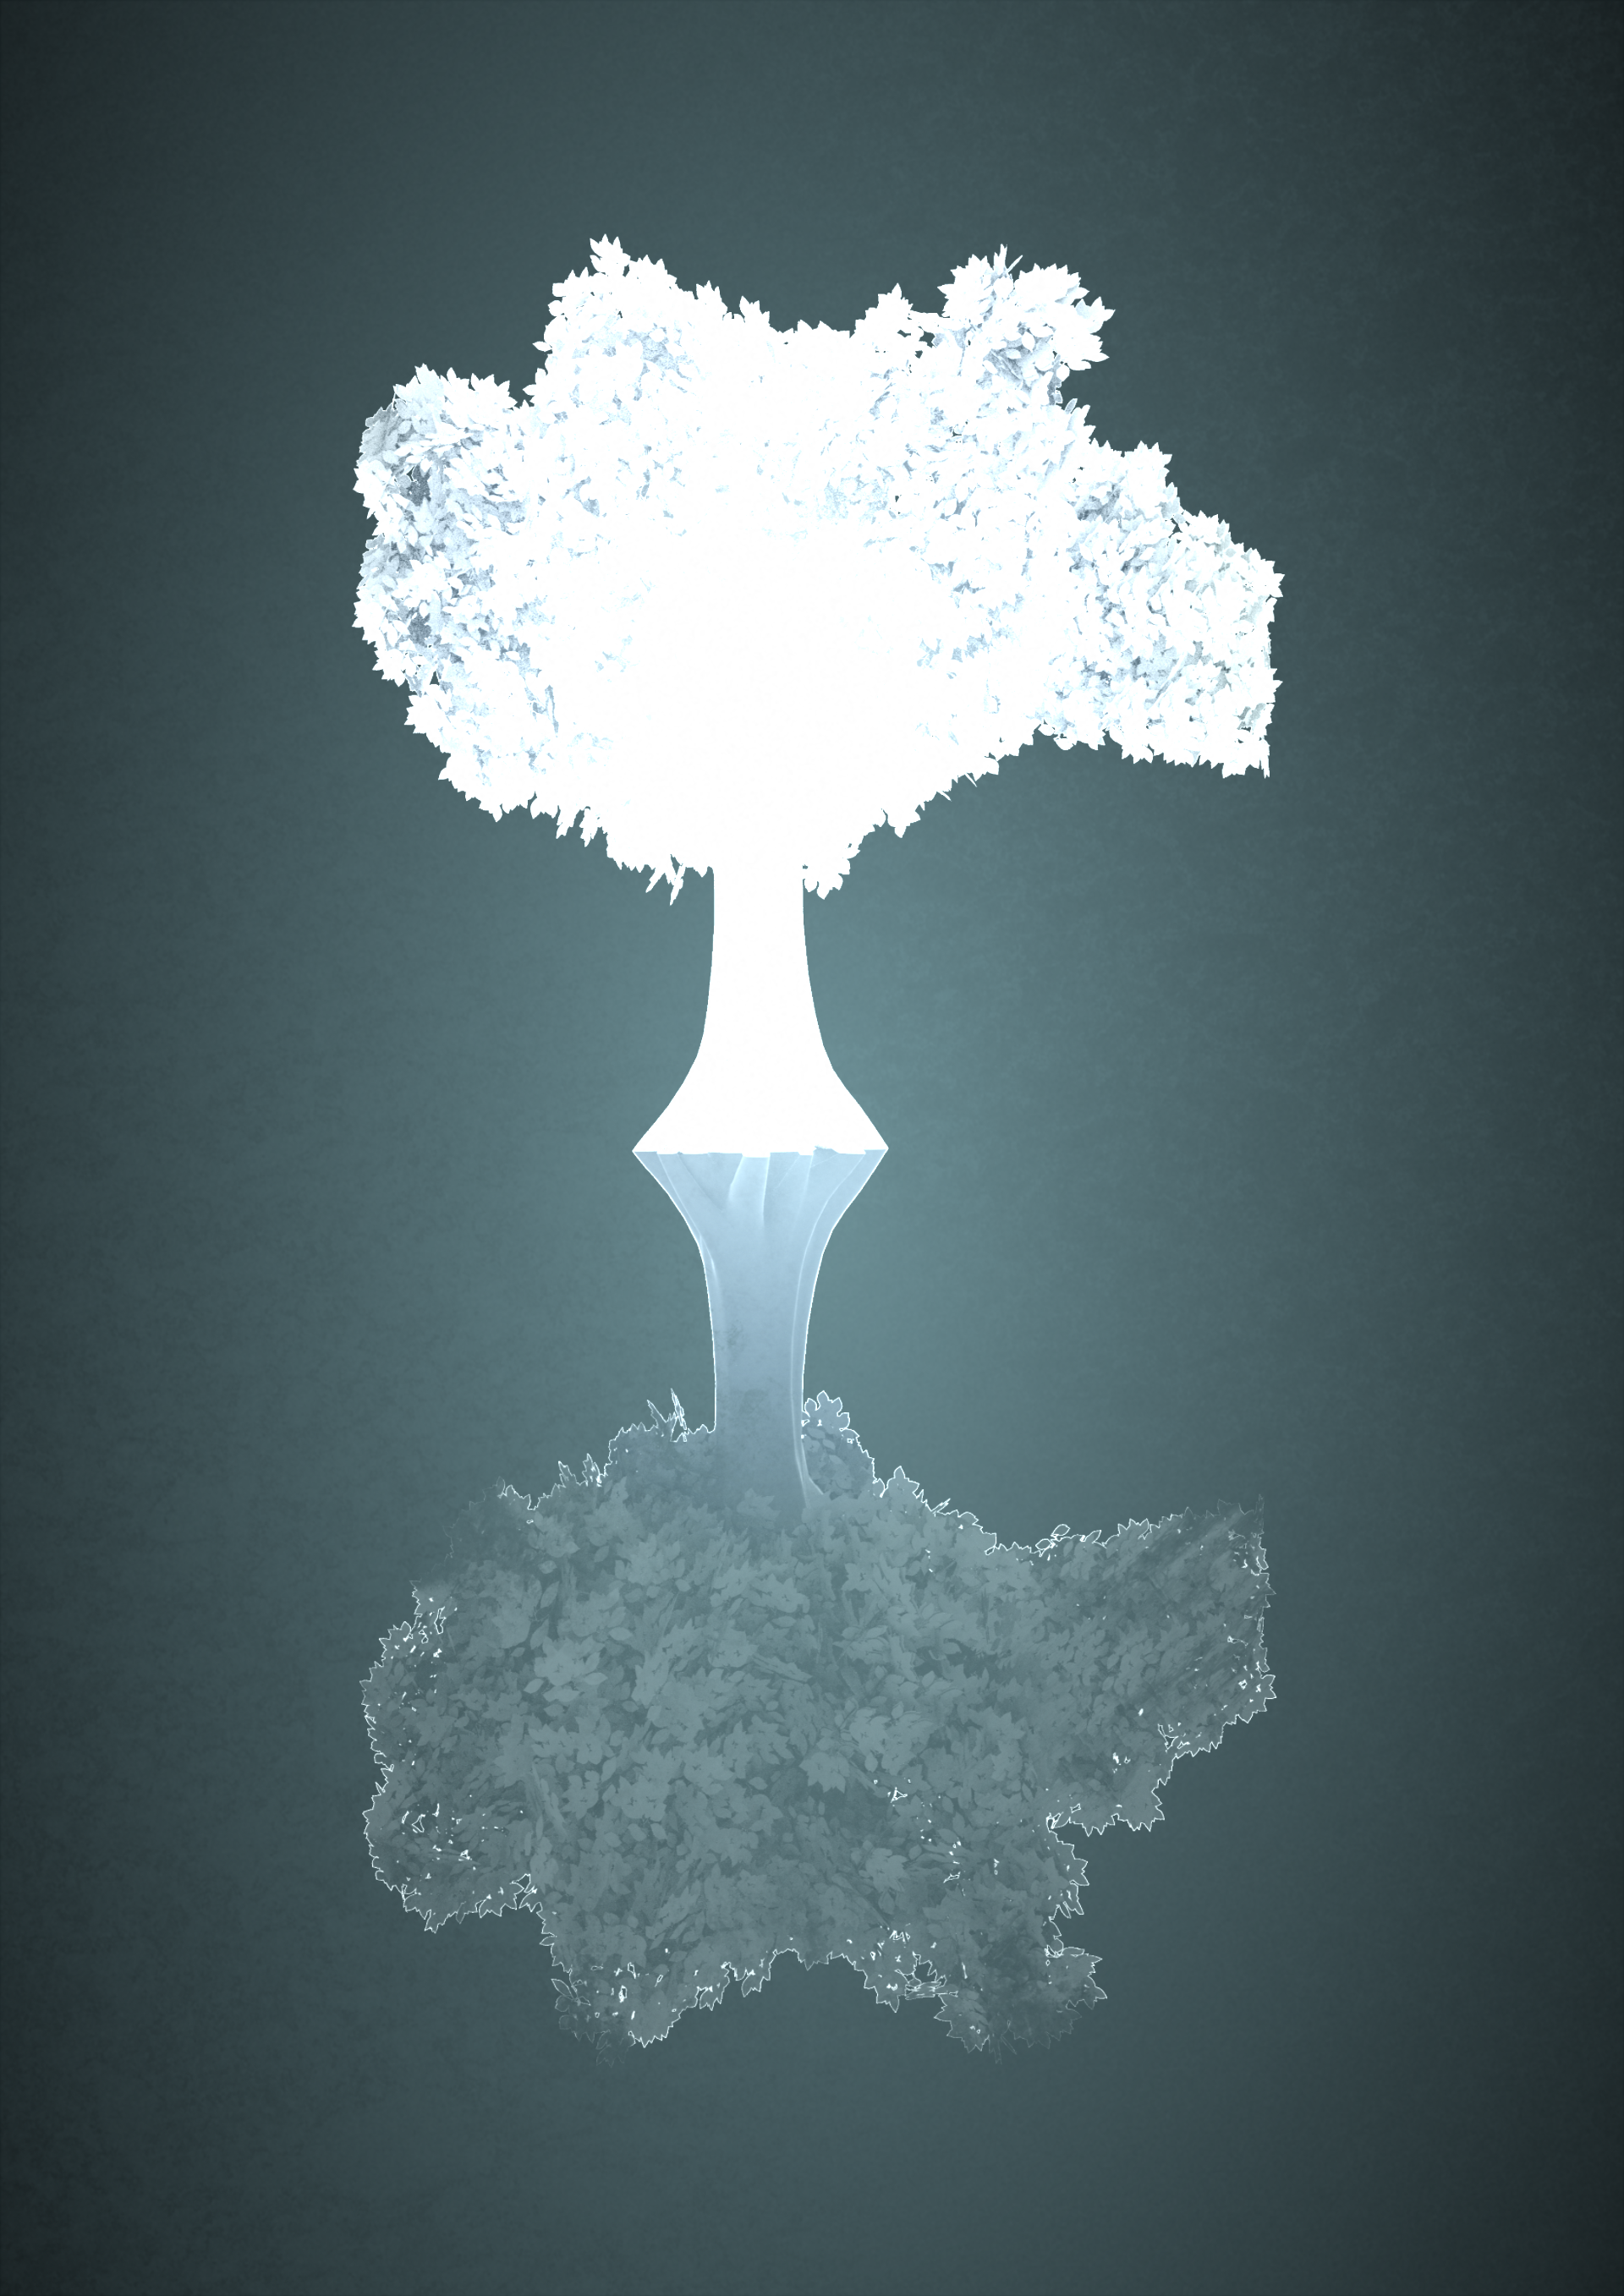
\includegraphics[scale=0.055]{img/front.png}
}
\SetBgOpacity{1}
\BgThispage

\newpage
\noindent \textbf{Steffan Sølvsten}

Aarhus, Denmark

\href{mailto:steffan.soelvsten@hotmail.com}{steffan.soelvsten@hotmail.com}

\vspace{1em}
\noindent Project started 2018

\vspace{1em}
\noindent Permission is hereby granted, free of charge, to any person obtaining a copy of
the document source files (the "Document"), to deal in the Document without
restriction, including without limitation the rights to use, copy, modify,
merge, publish, distribute and/or sublicense copies of the Document, and to
permit persons to whom the Document is furnished to do so, subject to the
following conditions:

The above copyright notice and this permission notice shall be included in all
copies or substantial portions of the Document. 

THE DOCUMENT IS PROVIDED "AS IS", WITHOUT WARRANTY OF ANY KIND, EXPRESS OR
IMPLIED, INCLUDING BUT NOT LIMITED TO THE WARRANTIES OF MERCHANTABILITY, FITNESS
FOR A PARTICULAR PURPOSE AND NONINFRINGEMENT. IN NO EVENT SHALL THE AUTHORS OR
COPYRIGHT HOLDERS BE LIABLE FOR ANY CLAIM, DAMAGES OR OTHER LIABILITY, WHETHER
IN AN ACTION OF CONTRACT, TORT OR OTHERWISE, ARISING FROM, OUT OF OR IN
CONNECTION WITH THE SOFTWARE OR THE USE OR OTHER DEALINGS IN THE SOFTWARE. 

\vspace{2em}
% https://tex.stackexchange.com/questions/128636/center-hrule-in-the-middle-of-the-page
\noindent\hfil\rule{0.8\textwidth}{.4pt}\hfil

\vspace{2em}
\noindent This book has been created as a joined group effort of the students of Aarhus
University. Thanks to everyone who has contributed with smaller og bigger
sections, corrections, feedback, proof-reading and much more.
  
\begin{multicols}{2}
  Johannes Ernstsen

  \hfill
  \columnbreak
  
  Kira Kutscher
\end{multicols}
}

\newpage
\thispagestyle{empty} % remove header and footer
\tableofcontents

\newpage
%%%%%%%%%%%%%%%%%%%%%%%%%%%%%%%%%%%%%%%%%%%%%%%%%%%%
% Chapter: Introduction
\section{Introduction}
\label{sec:introduction}

This section consists of different real-life examples, which exemplify one or more concepts defined in section \ref{sec:1} and are hence also grouped into equivalent sections.

\newpage
%%%%%%%%%%%%%%%%%%%%%%%%%%%%%%%%%%%%%%%%%%%%%%%%%%%%
% Chapter: Theory and Concepts
\setcounter{page}{1}

\section{Theory}
\label{sec:1}

In this section all frameworks, concepts and methods will be defined, compared and criticised. They are simultaneously grouped into the point in development they are to be used.

Today design of interactive systems is centered around the end user and constant reevaluation, which the Y-Model in framework \ref{fw:y_model} reflects perfectly.

\begin{framework}[Y-Model] \label{fw:y_model} \index{Y-Model}
  
\end{framework}


\subsection{Underlying Concepts}
\label{sec:1_concepts}
This section contains theory and concepts underlying all the following sections.

\begin{definition}[Tacit Knowledge] \label{def:tatic_knowledge} \index{Tacit Knowledge}
  Knowledge a person has and uses, but is unable to put in words or in other ways explain or pass on to others.
\end{definition}


\subsection{Agile Development}
\label{sec:1_agile}


\begin{concept}[Agile Method] \label{conc:agile} \index{Agile Method}
  
\end{concept}

\subsubsection{Scrum}

\begin{definition}[Product Owner] \label{def:product_owner} \index{Product Owner}

\end{definition}

\begin{definition}[Scrum Master] \label{def:scrum_master} \index{Scrum Master}

\end{definition}

\begin{definition}[Product Backlog] \label{def:product_backlog} \index{Product Backlog}

\end{definition}

\begin{definition}[Sprint] \label{def:sprint} \index{Sprint}

\end{definition}

\begin{definition}[Sprint Backlog] \label{def:sprint_backlog} \index{Sprint Backlog}

\end{definition}

\begin{definition}[Daily Scrum] \label{def:daily_scrum} \index{Daily Scrum}

\end{definition}

\begin{definition}[Sprint Review and Retrospective]  \label{def:sprint_review} \index{Sprint Review and Retrospective}

\end{definition}


\subsection{Stages of design}
The grouping of methods, concepts and more makes it seem like the design process is a linear process, which it should not be at all. The design process should as much as possible follow the idea of agile development in section \ref{sec:1_agile}. This means, that no section is ever properly finished, as the designer will keep on going back, but rather the next section is also juggled together with the prior things at the same time.

\subsubsection{Initial}
\label{sec:1_initial}

\begin{framework}[PACT] \label{fw:pact} \index{PACT Framework}
  
\end{framework}
\subsubsection{Data Gathering}
\label{sec:1_data_gathering}

\begin{concept}[Interview] \label{conc:interview} \index{Interview}

  
\end{concept}

\subparagraph{Structured Interview / Survey} \index{Structured Interview} \index{Survey}


\subparagraph{Semistructured Interview} \index{Semistructured Interview}


\subparagraph{Unstructured Interview} \index{Semistructured Interview}


\begin{method}[Observation] \label{meth:observation} \index{Observation}
  
\end{method}

\begin{method}[Contextual Interview] \label{meth:contextual_interview} \index{Contextual Inteview}
  
\end{method}

\begin{definition}[Artifact] \label{def:artifact} \index{Artifact}
  
\end{definition}

\begin{method}[Artifact Gathering] \label{meth:artifact_collection} \index{Artifact Collection}
  Collecting artifacts either physically or by taking picture of them, if you are unable to retreive the artifact from the site.
\end{method}
\subsubsection{Data Analysis}
\label{sec:1_data_analysis}
The main purpose of the data analysis step is to take the data gathered and extract conclusions about the system to be designed. After having done the analysis, criteria for the system to be designed will be clear to the designer. Furthermore in this step a lot of tools such as personas and user stories are created, which are valuable tools in the later design process.

Since always more knowledge is gained around the field for which you design, it is normal to turn back to this stage quite a lot to redo or add to prior work.

\begin{method}[Affinity Diagram] \label{meth:affinity_diagram} \index{Affinity Diagram}
  
\end{method}

\begin{method}[Rich Picture] \label{meth:rich_picture} \index{Rich Picture}
  
\end{method}

\begin{tool}[Persona] \label{tool:persona} \index{Persona}
  
\end{tool}

\begin{tool}[User Stories (Scenario)] \label{tool:user_stories} \index{User Stories (Scenario)}
  
\end{tool}

\begin{figure}
  \centering
  % TODO : Recreate the figure from Benyon
  \caption{The four different types of scenarios \cite[p. 67]{benyon_14}}
  \label{fig:scenarios}
\end{figure}

\begin{definition}[Flow Model] \label{meth:flow_model} \index{Flow Model}
  
\end{definition}

\begin{definition}[Sequence Model] \label{meth:sequence_model} \index{Sequence Model}
  
\end{definition}

\subsubsection{Envisionment}
\label{sec:1_envisionment}

\begin{method}[Individual Snapshot] \label{meth:individual_snapshot} \index{Individual Snapshot}
  
\end{method}

\begin{tool}[Storyboard] \label{meth:storyboard} \index{Storybaord}
  
\end{tool}

\begin{tool}[Conceptual Scenario] \label{meth:conceptual_scenario} \index{Conceptual Scenario}
  This is based on Benyon
\end{tool}

\begin{tool}[Conceptual Model] \label{def:conceptual_model} \index{Conceptual Model}
  
\end{tool}

\begin{definition}[Metaphor] \label{def:metaphor} \index{Methaphor}
  
\end{definition}

\begin{definition}[Design Language] \label{def:design_language} \index{Design language}
  
\end{definition}

\begin{tool}[Navigation Map] \label{meth:navigation_map} \index{Navigation Map}
  
\end{tool}

\begin{tool}[Mood Board] \label{tool:mood_board} \index{Mood Board}
  
\end{tool}


\subsubsection{Prototyping}
\label{sec:1_prototyping}



\begin{method}[Concrete Scenario] \label{meth:concrete_scenario} \index{Concrete Scenario}
  
\end{method}

\begin{method}[Use Cases (Scenario)] \label{meth:use_cases} \index{Use Cases (Scenario)}
  
\end{method}

\begin{definition}[Lo-Fi Prototype] \label{def:lo-fi_prototype} \index{Lo-Fi Prototype}
  
\end{definition}

\begin{definition}[Hi-Fi Prototype] \label{def:hi-fi_prototype} \index{Hi-Fi Prototype}
  
\end{definition}

\begin{method}[Evaluation of prototypes] \label{meth:evaluation_of_prototypes} \index{Evaluation of Prototypes}
  
\end{method}

\newpage
%%%%%%%%%%%%%%%%%%%%%%%%%%%%%%%%%%%%%%%%%%%%%%%%%%%% 
% Chapter: Examples
\section{Examples}
\label{sec:2}

This section consists of different real-life examples, which exemplify one or more concepts defined in section \ref{sec:1} and are hence also grouped into equivalent sections.
% TODO: Add sections
%       Need to know structure of part 1 first

\newpage
%%%%%%%%%%%%%%%%%%%%%%%%%%%%%%%%%%%%%%%%%%%%%%%%%%%% 
% Chapter: Exercises
\section{Exercises}
\label{sec:3}

This section consists of different exercises, such that you can try to apply the theory from section \ref{sec:1} in small isolated cases written up for maximizing your learning outcome. These exercises are grouped into subsections in relation to the subsections in \ref{sec:1}.
% TODO: Add sections
%       Need to know structure of part 1 first


\newpage
%%%%%%%%%%%%%%%%%%%%%%%%%%%%%%%%%%%%%%%%%%%%%%%%%%%% 
% References
\begin{minipage}{1.0\textwidth}
  \begin{thebibliography}{9}
  \bibitem{benyon_14}
    Benyon, David: \emph{Designing Interactive Systems}, Pearson, 3rd edition, 2014
  \bibitem{benyon_10}
    Benyon, David: \emph{Designing Interactive Systems}, Pearson, 2nd edition, 2010
  \bibitem{rogers}
    Rogers, Yvonne: \emph{Interaction Design: Beyond human-computer interaction}, Wiley, 3rd edition, 2011
  \bibitem{lim}
    Lim, Youn-Kyung and Tenenberg, Josh: \emph{The Anatomy of Prototypes}, ACM Transactions on Computer-Human Interaction, Vol. 15, 2008
  \end{thebibliography}
  \bibliographystyle{abbrv}
  \bibliography{referencer}
\end{minipage}

\newpage
%%%%%%%%%%%%%%%%%%%%%%%%%%%%%%%%%%%%%%%%%%%%%%%%%%%% 
% Index
\printindex

\newpage
%%%%%%%%%%%%%%%%%%%%%%%%%%%%%%%%%%%%%%%%%%%%%%%%%%%% 
% Backcover
\thispagestyle{empty} % remove header and footer
\begin{center}
  \begin{minipage}[r]{0.6\linewidth}
    \phantom{}\vspace{2.7cm}
    \begin{abstract}
      \noindent After having to read three different books on Human Computer Interaction, this is an attempt to dispose of the frustrating amount of unecessary information and vague or non-existent definitions in the HCI universe apparent in all these text books. This is to be a dense, clearly defined, and small guide to interaction design
    \end{abstract}  
  \end{minipage}  
\end{center}

\SetBgContents{
    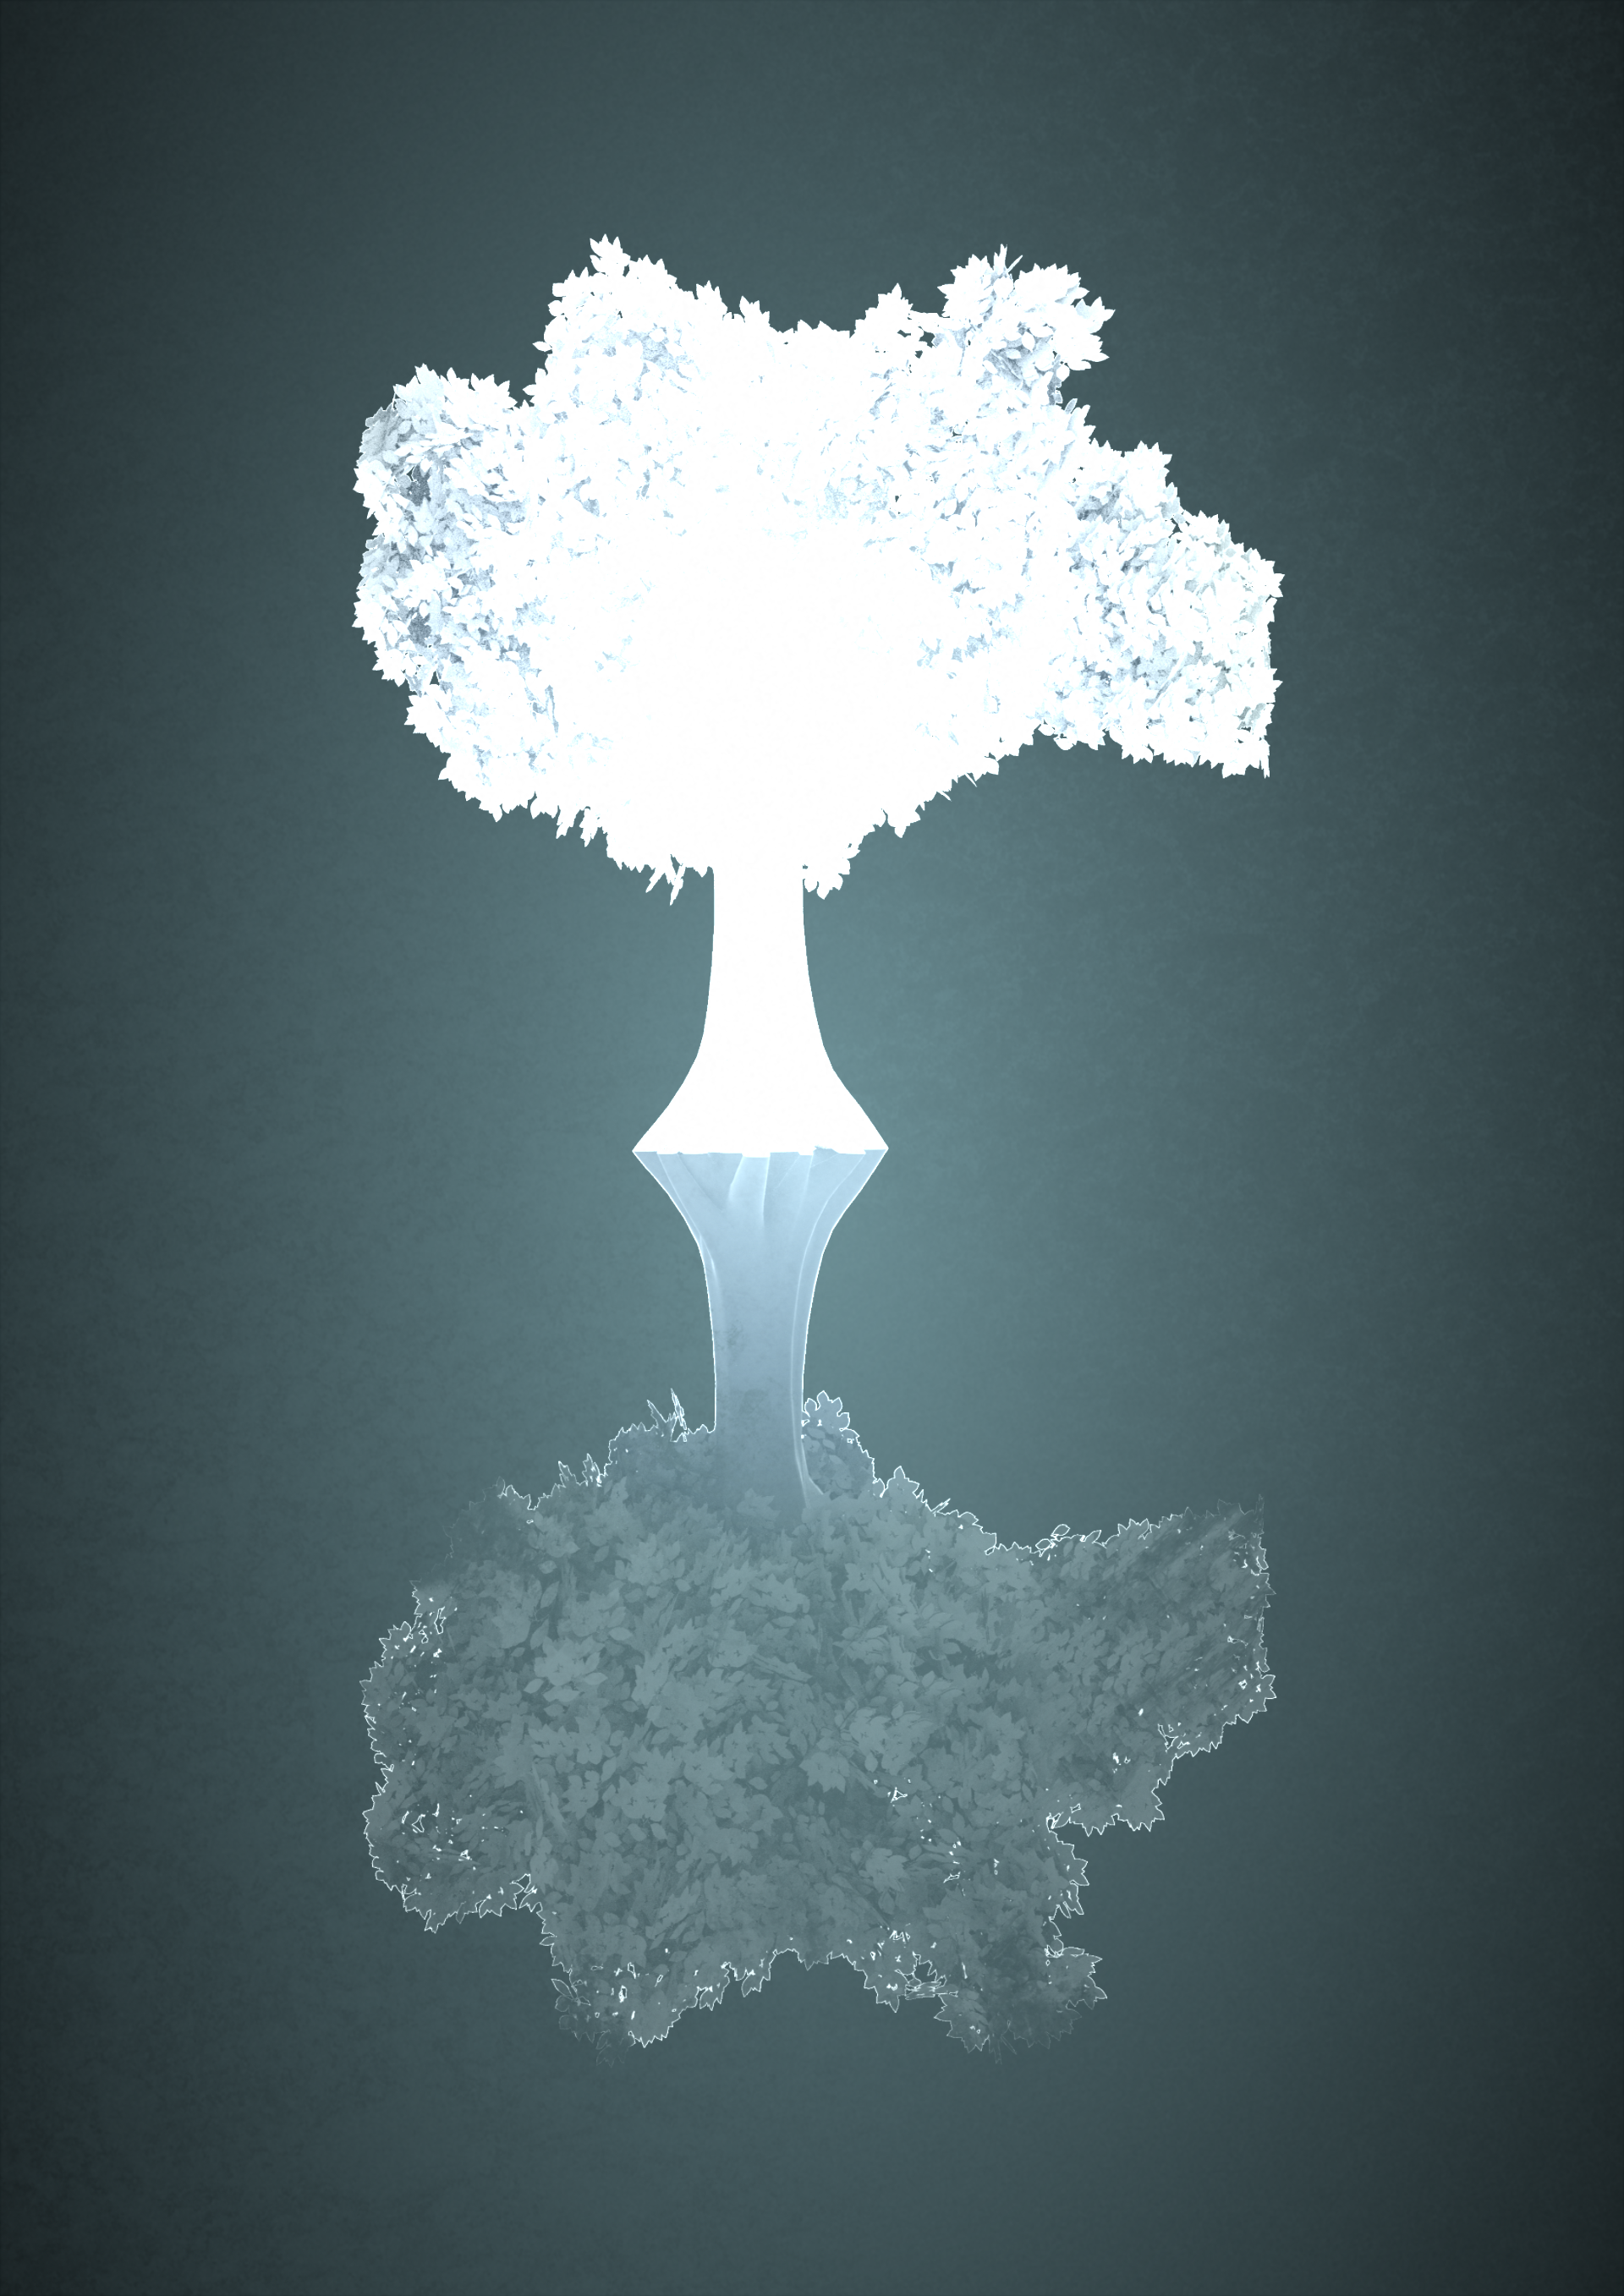
\includegraphics[scale=0.055]{img/front.png}
}
\SetBgOpacity{1}
\BgThispage

\end{document}
